%%%%%%%%%%%%%%%%%%%%%%%%%%%%%%%%%%%%%%%%%%%%%%%%%%%%%%%%%%%%%%%%%%%%%%
%%                                                                 %%
%% Please do not use \input{...} to include other tex files.       %%
%% Submit your LaTeX manuscript as one .tex document.              %%
%%                                                                 %%
%% All additional figures and files should be attached             %%
%% separately and not embedded in the \TeX\ document itself.       %%
%%                                                                 %%
%%%%%%%%%%%%%%%%%%%%%%%%%%%%%%%%%%%%%%%%%%%%%%%%%%%%%%%%%%%%%%%%%%%%%

\documentclass[sn-mathphys,Numbered, lineno]{sn-jnl}  % I added lineo to have linenumbers

%%%% Standard Packages
%%<additional latex packages if required can be included here>
\usepackage{graphicx}%
\usepackage{multirow}%
\usepackage{amsmath,amssymb,amsfonts}%
\usepackage{amsthm}%
\usepackage{mathrsfs}%
\usepackage[title]{appendix}%
\usepackage{xcolor}%
\usepackage{textcomp}%
\usepackage{manyfoot}%
\usepackage{booktabs}%
\usepackage{algorithm}%
\usepackage{algorithmicx}%
\usepackage{algpseudocode}%
\usepackage{listings}%

%%%%
% REMOVE THOSE IN THE END
\usepackage{todonotes}
\usepackage{caption}
\usepackage{tabularx}
\usepackage{adjustbox}  % for the adjustwidth


%\jyear{2021}%

%% as per the requirement new theorem styles can be included as shown below
\theoremstyle{thmstyleone}%
\newtheorem{theorem}{Theorem}%  meant for continuous numbers
%%\newtheorem{theorem}{Theorem}[section]% meant for sectionwise numbers
%% optional argument [theorem] produces theorem numbering sequence instead of independent numbers for Proposition
\newtheorem{proposition}[theorem]{Proposition}% 
%%\newtheorem{proposition}{Proposition}% to get separate numbers for theorem and proposition etc.

\theoremstyle{thmstyletwo}%
\newtheorem{example}{Example}%
\newtheorem{remark}{Remark}%

\theoremstyle{thmstylethree}%
\newtheorem{definition}{Definition}%

\raggedbottom
%%\unnumbered% uncomment this for unnumbered level heads

\begin{document}

\title[Article Title]{
    Genomic, metabolic and literature oriented annotation of microbial co-occurrence networks 
    enhances associations confidence level and hypothesis generation
}


\author[1]{\fnm{Haris} \sur{Zafeiropoulos}}\email{haris.zafeiropoulos@kuleuven.be}
\author[1]{\fnm{Ermis Ioannis} \sur{Michail Delopoulos}}\email{ermisioannis.michaildelopoulos@student.kuleuven.be}
% \equalcont{These authors contributed equally to this work.}
\author[2]{\fnm{Andi} \sur{Erega}}\email{andi.erega@hest.ethz.ch}
% \equalcont{These authors contributed equally to this work.}
\author[2]{\fnm{Annelies} \sur{Geirnaert}}\email{annelies.geirnaert@hest.ethz.ch}
\author[3]{\fnm{John} \sur{Morris}}\email{scooter@cgl.ucsf.edu}
\author*[1]{\fnm{Karoline} \sur{Faust}}\email{karoline.faust@kuleuven.be}


\affil*[1]{
    \orgdiv{
        Department of Microbiology, Immunology and Transplantation, Rega Institute for Medical Research
    }, 
    \orgname{KU Leuven}, 
    \orgaddress{
        \street{Herestraat}, \city{Leuven}, \postcode{3000}, \state{}, \country{Belgium}
    }
}
\affil[2]{
    \orgdiv{Institute of Food, Nutrition and Health}, 
    \orgname{ETH Zurich}, 
    \orgaddress{
        \street{Street}, \city{Zurich}, \postcode{8092}, \state{}, \country{Switzerland}
    }
}
\affil[3]{
    \orgdiv{Department of Pharmaceutical Chemistry}, 
    \orgname{University of California San Francisco}, 
    \orgaddress{
        \street{Street}, \city{San Francisco}, \postcode{94143}, \state{California}, \country{USA}
    }
}


%%==================================%%
%% unstructured abstract %%
%%==================================%%
\abstract{

    Up to 350 words.

    The abstract must include the following separate sections:
    
    \textbf{Background:} the context and purpose of the study

    \textbf{Results:} the main findings

    \textbf{Conclusions:} a brief summary and potential implications


    \begin{figure}[H]
        \label{fig:abstract}
        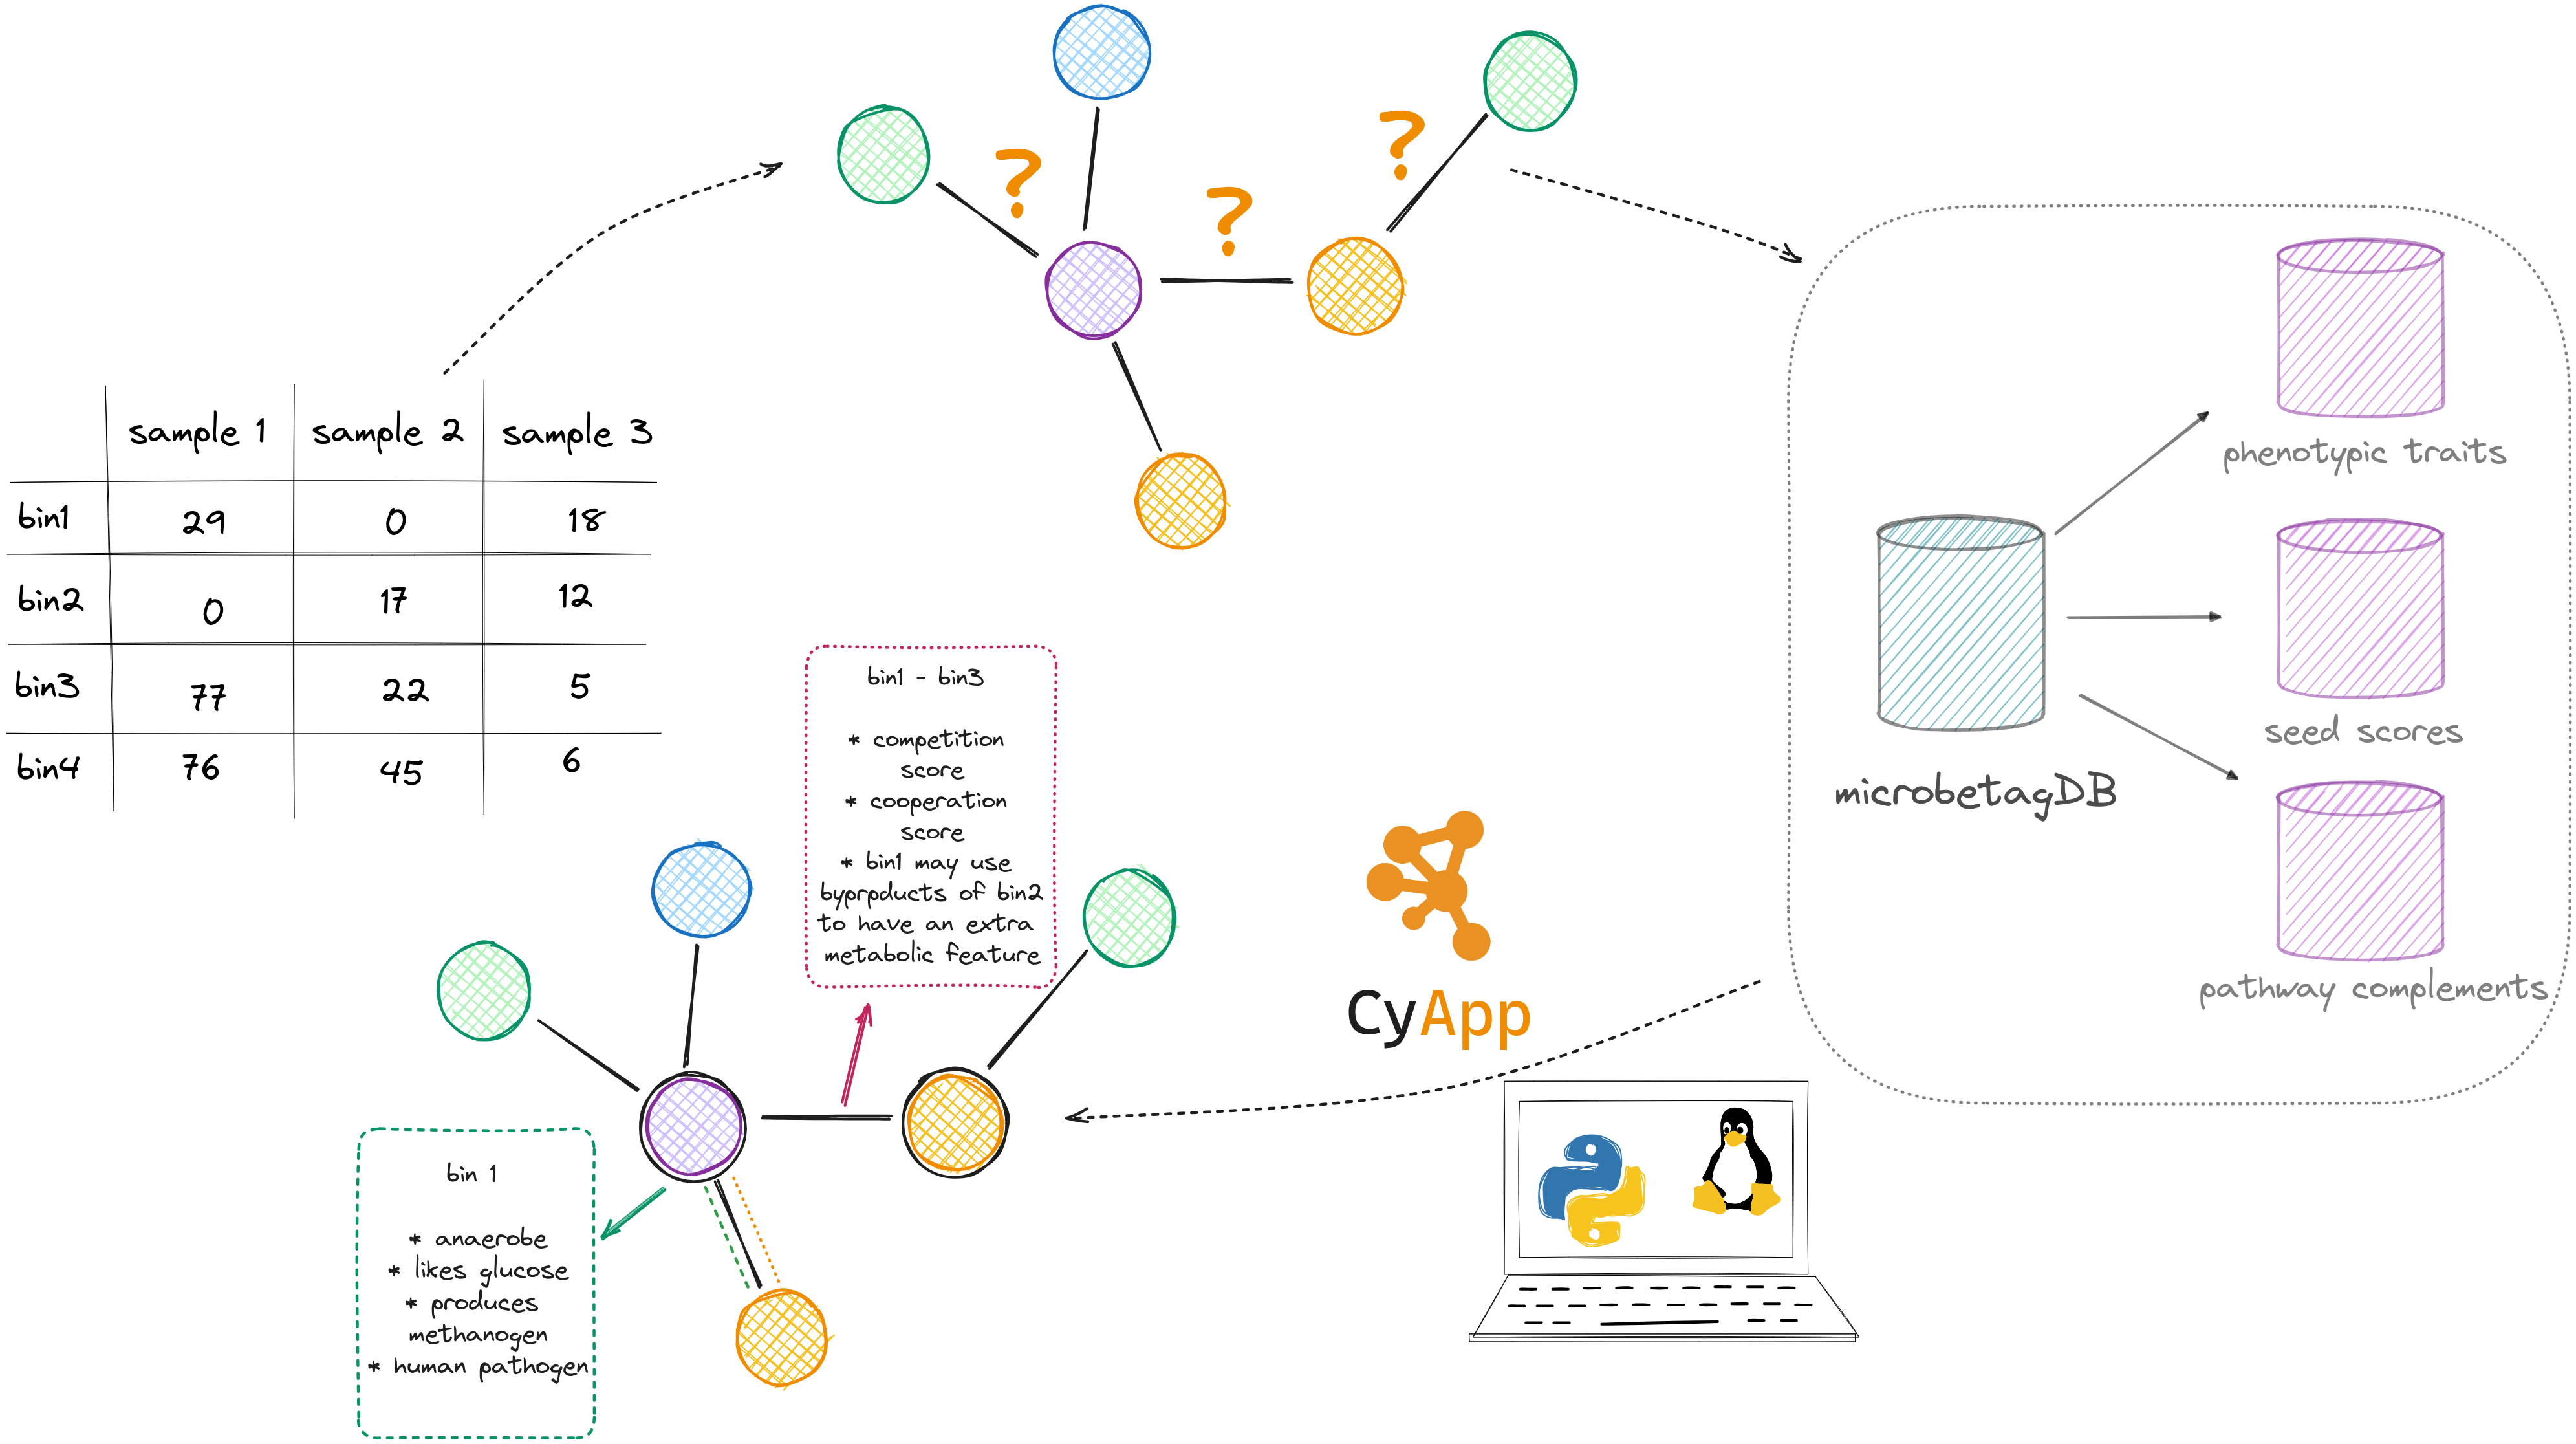
\includegraphics[width=\columnwidth]{figs/figure_abstract.png}
        \caption*{
            Figure abstract. 
            
            % From a count table (bins or OTUs/ASVs) one can come up with a co-occurrence network. 
            % To better understand and assess the confidence level of these associations, microbetag annotates both taxa (nodes) 
            % and 
            % integrating 
            % genomic data 
            
        }
    \end{figure}
    

}
%%==================================%%
%% keywords                         %%
%%==================================%%
\keywords{
    microbial associations, 
    enrichemnt analysis, 
    data integration,
    pathway complementarity,
    seed set
}



\maketitle


%%==================================%%
%% MAIN BODY                        %%
%%==================================%%

\section{Introduction}
\label{sec1}

    \footnote{
        We are to submit in the Microbiome journal as a "Software" manuscript, thus we follow
        ~\href{https://microbiomejournal.biomedcentral.com/submission-guidelines/preparing-your-manuscript/software-article}{these rules}
    }
    \footnote{The introduction should not include subheadings.}

    % SKELETON FOR THE Introduction
    \hrulefill
    \begin{itemize}
        \item Role of microbial associations in the study of microbial communities
        \item HTP sequencing 
        \item cooccurrence networks to analyse HTP data
        \item challenges of cooccurrence networks / refs:
            ~\cite{berry2014deciphering}: microbial network inference as a tool for interaction prediction has highlighted this tool’s low accuracy and the biological implications of network properties are unclear /
            \cite{ma2020earth} :  modules in microbial co-occurrence networks may be indicative of ecological processes governing community structure, such as niche filtering and habitat preference
        
        \item current approaches to deal with those challenges
        \item our contribution 
    \end{itemize}

    \hrulefill

    It is well known that most microbial species live not in isolation but in communities~\cite{rottjers2018hairballs}.
    Such communities play a crucial role in ecosystem functioning in almost any ecosystem type~\cite{raes2008molecular, faust2012microbialReviewInteractions}.
    High-throughput sequencing (HTP) has provided great insight into the diversity and composition of microbial communities~\cite{elixir_microbiome}. % get more refs
    Uncultivated species can now be detected and their featues can be inferred through their genomic information~\cite{hug2016new}.

    NGS facilitates culture-independent sampling of the microorganisms in an area with the potential for both taxonomic and functional annotation;


    NGS not only provides information about the taxonomic composition of the microbial community but also enables the annotation of their functional capabilities. 
    This combination of taxonomic and functional annotation provides a more detailed and holistic view of the role and activities of microorganisms.




    



    Understanding the structure, composition, and dynamics of microbial communities is crucial for unraveling the intricate web of interactions that shape ecosystems. 
    To come up with a comprehensive understanding of these interactions, we need to comprehend the relationships between microorganisms and thus their own interactions.

    The notion of an interaction varies including cooperation, competition, parasitism, commensalism and ammensalism~\cite{faust2012microbialReviewInteractions}.



    Microbial interactions play a crucial role in shaping ecosystems and influencing various biological processes. 

    
    These interactions contribute to the overall stability and functioning of ecosystems by influencing nutrient cycling, disease dynamics, and the overall diversity and composition of microbial communities. 
    For example, some microorganisms can produce and release certain compounds that benefit neighboring microbes or inhibit the growth of competing species. 
    Other interactions involve symbiotic relationships, where different microbes rely on each other for survival and perform complementary functions. 
    Understanding and studying microbial interactions is vital for unraveling the complexity of microbial communities and their impact on human health, agriculture, and environmental processes.


    Physical Interactions: Microorganisms can interact physically by forming biofilms, which are communities of microorganisms attached to surfaces and enclosed in a matrix of extracellular substances. Biofilms provide protection and promote cooperation among the microorganisms within them.

    Quorum Sensing: Many bacteria use quorum sensing to communicate with each other and coordinate their behavior. They release and detect signaling molecules called autoinducers, which allow them to sense the local population density. This mechanism enables bacteria to coordinate processes like biofilm formation, virulence factor expression, and nutrient acquisition.
    
    Antibiosis: Antibiosis refers to the production of antimicrobial substances by microorganisms that inhibit the growth or survival of other microorganisms. This can be a competitive strategy to gain an advantage in a particular environment.
    
    metabolic interactions specifically, microorganisms often engage in metabolic exchanges during their interactions. For instance, one microbe may produce metabolites that serve as nutrients or signaling molecules for another microbe. These metabolic interactions can involve the transfer of essential nutrients, the breakdown of complex compounds, or the production of secondary metabolites with antimicrobial properties.
    Overall, understanding the different types of microbial interactions, including metabolic interactions, provides insights into the complexity and dynamics of microbial communities and their impact on various processes in nature.






    A widely used approach is the creation of co-occurrence networks based on community data. To build such networks, there is a great number of approaches: Spearman and Pearson correlations, CoNet~\cite{faust2012microbial} SparCC~\cite{friedman2012inferring} SpiecEasi~\cite{kurtz2015sparse}, MAGMA~\cite{cougoul2019magma} and FlashWeave~\cite{flashweave_cite} are just a few of them.
    However, the outcome is usually tool-dependent~\cite{kishore2023inferring, weiss2016correlation, rottjers2018hairballs}. 

    Metagenomic or metabarcoding data are often used to predict microbial interactions in complex communities, but these predictions are rarely explored experimentally and/or validated. 

    FlashWeave 

    microbeAnnotator~\cite{ruiz2021microbeannotator} 


    Related literature:
    Karaoz U and Brodie EL (2022) microTrai~\cite{karaoz2022microtrait} , a computational pipeline that infers and distills ecologically relevant traits from microbial genome sequences.
    It does not apply networks









\section{Implementation}
\label{sec:implementation}

    \footnote{This should include a description of the overall architecture of the software implementation, along with details of any critical issues and how they were addressed.}

    \subsection*{Genomes included}
    \label{subsec:genomes}

        Using the GTDB v202 \href{https://data.gtdb.ecogenomic.org/releases/release202/202.0/}{metadata files}, we retrieved the NCBI genome accessions of the representative genomes of high quality, i.e. completeness $\geq 95\%$  and contamination $\leq 5\%$.
        That resulted a set of $26,778$ covering $22,009$ unique NCBI Taxonomy Ids.
        Using these accession numbers, we were able to download their corresponding \texttt{.faa} files when available (\href{https://github.com/hariszaf/microbetag/blob/develop/microbetagDB/mappings/gtdb_ncbi/get_gtdb_faa.py}{\texttt{get\_gtdb\_faa.py}}) leading to a set of $16,900$ amino acid sequence files.
        % | genomes category | # of genomes|
        % |:-----:|:-------:|
        % |All GTDB  | 258,407 | 
        % | Representatives | 47,894 |
        % | High quality represntative | 26,778* | 
        % | HQ representative with `.faa` | 16,900** |


    \subsection*{Taxonomy schemes}
    \label{subsec:taxonomies}

        microbetag maps the taxonomy of each entry in the abundance table to its corresponding NCBI Taxonomy id and if available its closest GTDB representative genome(s).
        Two well established taxonomy schemes are supported.
        The Genome Taxonomy DataBase (GTDB)~\cite{parks2022gtdb} that is being broadly used in bins and/or MAGs taxonomical classification
        and the Silva database~\cite{quast2012silva} that has 
        NCBI Taxonomy~\cite{schoch2020ncbi}. 
        The primer links the representative genomes included to their corresponding NCBI Taxonomy ids too. 
        
        There is a great number of taxonomies that are being used in such studies, e.g. Silva~\cite{quast2012silva}, Ribosomal Database Project (RDP)~\cite{cole2014ribosomal}, manually curated ones and more, 
        As a consequence, there is not a standardised format of the taxonomies assigned, from bioinformatics pipelines used for the analysis of such data.
        microbetag makes use of the~\href{https://github.com/seatgeek/thefuzz}{\texttt{fuzzywuzzy}} library that implements the Levenshtein Distance Metric to get the closest NCBI taxon name and thus its corresponding NCBI Taxonomy id. 
        ++ ncbi nodes dump
        A relatively high similarity score is used (90) to avoid false positives. 



        DADA2 formatted 16S rRNA gene sequences for both bacteria and archaea~\cite{ali_alishum_2022_6655692} were used to trained the TAXID classifier~\cite{{murali2018idtaxa}} of the DECIPHER package.




    \subsection*{ Network inference }
    \label{subsec:net-infer}

        FlashWeave~\cite{flashweave_cite}

        a computational approach based on a flexible Probabilistic Graphical Model framework that integrates metadata and predicts direct microbial interactions from heterogeneous microbial abundance data sets with hundreds of thousands of samples. 

        A flexible Probabilistic Graphical Model framework is used in a computational approach that 
        incorporates metadata and predicts direct microbial interactions. 
        This is done using heterogeneous microbial abundance datasets consisting of hundreds of thousands of samples.

        %     •    heterogeneous - enable heterogeneous mode for multi-habitat or -protocol data with at least thousands of samples (FlashWeaveHE)
        %     •    sensitive - enable fine-grained associations (FlashWeave-S, FlashWeaveHE-S), sensitive=false results in the fast modes FlashWeave-F or FlashWeaveHE-F
        %     •    FDR - perform False Discovery Rate correction (Benjamini-Hochberg method) on pairwise associations
        %     •    n_obs_min - don't compute associations between variables having less reliable samples (i.e. non-zero if heterogeneous=true) than this number. -1: automatically choose a threshold.




    \subsection*{ Literature oriented node annotation }
    \label{subsec:fapro}

        Using a set of Tara Oceans samples~\cite{sunagawa2015structure} FAPROTAX~\cite{louca2016decoupling} estimates the functional potential of the bacterial and archaeal communities, by classifying each taxonomic unit into functional group(s) based on current literature,
        announcements of cultured representatives and/or manuals of systematic microbiology. 
        In this manually curated approach, a taxon is associated with a function if and only if all the cultured species within the taxon have been shown to exhibit that function. 
        % Apparently, FAPROTAX does not support the annotation of clades with no cultured representatives that have been rising thanks to high throughput sequencing technologies.
        % Further, a taxon could be annotated with more than one functions while functional groups could be nested.
        In its current version, FAPROTAX includes more than 80 functions based on ~7600 functional annotations and covering more than 4600 taxa.
        Contrary to gene content based approaches, e.g. PICRUSt2, FAPROTAX  estimates metabolic phenotypes based on experimental evidence. 

        microbetag invokes the accompanying script of FAPROTAX and converts the taxonomic microbial community profile of the samples included in the user's abundance table or of the taxa present in the provided network, into putative functional profiles.
        Then, it parses FAPROTAX's subtables to annotate each taxonomic unit present on the user's data with all the functions for which they had a hit. 
        FAPROTAX annotations are not part of the microbetagDB but are computed on the fly.


    \subsection*{ Genomic oriented node annotation }
    \label{subsec:phen}

        phenDB~\cite{feldbauer2015prediction} is a publicly available resource that supports the analysis of bacterial (meta)genomes to identify 47 distinct functional traits. 
        It relies on support vector machines (SVM) trained with manually curated datasets based on gene presence/absence patterns for trait prediction.
        More specifically, the model for a particular trait is trained using a collection of EggNOG annotated genomes where the knowledge of whether that trait is present or absent among its members is available.
        The \texttt{compute-genotype} program of phenotrex supports the creation of such tabular \textit{genotype} files.
        A \textit{genotype} file can be used along with a~\textit{phenotype} one, i.e., a file containing true phenotypic trait values for each input genome on which to train the model, and the \texttt{train} program of phenotrex can then be performed. 
        % one can implement tests to evaluate the model based on the completeness of a genomes and its contamination (Performance Estimation) using the cccv program. e.g
        % {
        % 	"mean_balanced_accuracy": 0.5499999999999999,
        % 	"stddev_balanced_accuracy": 0.10482201257840669,
        % 	"contamination": 0.7,
        % 	"completeness": 1.0
        % },
        Last, the models can now be used to predict their corresponding traits; based on the completeness/contamination of the genomes, the accuracy varies. 
        
        In the frameowrk of microbetagDB, phenotrex classifiers were re-trained using the genomes provided by phenDB for each trait to sync with the latest version of eggNOG. 
        Genomes were downloaded from NCBI using the \href{https://www.ncbi.nlm.nih.gov/sites/batchentrez}{Batch Entrez} program.
        % as there was a conflict between the eggNOG version phenotrex uses at the prediction step and the one during the training of the classes as provided in the PhenDB site.
        % For example, for the acetic acid production case, the corresponding webpage of phenDB pointed to the set of genomes that had been originally used. 
        Then, \textit{genotype} files were produced for all the high quality GTDB representative genomes.
        Each model was then used against all the GTDB \textit{genotype} files to annotate each with the presence or the absence of the trait. 




    \subsection*{ Pathway complementarity }
    \label{subsec:path-compl}

        For the subset of the 16,900 high quality GTDB representative genomes that a \texttt{.faa} was available, 
        \textit{kofamscan}~\cite{aramaki2020kofamkoala} was performed to annotate them with KEGG ORTHOLOGY terms (KOs)~\cite{kanehisa2012kegg}. 
        Their KOs were then mapped to their corresponding KEGG modules. 
        A KEGG module is defined as a functional unit within the KEGG framework, that represents a set of enzymes and reactions involved in a specific biological process or pathway~\cite{muto2013modular}.
        A module's definition is a logical expression and consists of KOs and the following symbols:
        a. the space, representing a connection in the pathway
        b. plus sign, representing a molecular complex,  
        c. comma, representing alternatives and
        d. minus sign, designates an optional item in the complex.
        Both (a) and (b) cases should be considered as "AND" logical operators, while (c) would be the "OR".

        \begin{figure}[h!]
        \label{fig:path-compl}
        \includegraphics*[width=0.8\columnwidth]{figs/path_complem.png}
        \caption{
            Pathway complementarity approach. 
            The high quality GTDB genomes were annotated with KEGG ORTHOLOGY (KO) terms.
            The various ways of getting a KEGG module complete were enumerated and all the possible ways a donor species could "fill" a beneficiary's non-complete module were calculated.
            In this case, there are 4 unique ways for having the serine biosynthesis module complete; in all of them K00831 is required.
            However, it is missing from the beneficiary species that supports the 2 out of the 3 steps of the module's definition.
            A donor species having and potentially sharing the corresponding enzyme of K00831 may enable the beneficiary species to produce serine.
        }
        \end{figure}

        We define a genome as having a "complete" module if and only if all of the KOs present in any of the module's alternatives are also found among the annotated KOs of the genome.
        All modules definitions were retrieved using the KEGG API and parsed 
        (\href{https://github.com/hariszaf/microbetag/blob/develop/microbetagDB/mappings/kegg_mappings/parse_module_definitions.py}{\texttt{parse\_module\_definitions.py}}).
        A dictionary was built with all the alternatives, i.e. alternative sets of KOs, for a module to be complete 
        (\href{https://github.com/hariszaf/microbetag/blob/develop/microbetagDB/mappings/kegg_mappings/module_definition_map.json}{module\_definition\_map.json}).
        Each pair of the KEGG annotated genomes was then investigated for potential pathway complementarities, 
        i.e. whether a genome lacking a number of KOs ($genome_A$) to have a complete module ($module_x$) could benefit from another's species genome(s) ($genome_B$).
        In that case, $genome_B$ does not necessarily have a complete alternative of $module_x$; as long as it has the missing KOs that $genome_A$ needs to complete an alternative of it, $genome_B$ potentially complements $genome_A$ with respect to $module_x$.
        In total, $341,568$ unique complementarities were exported (\href{https://github.com/hariszaf/microbetag/blob/develop/microbetagDB/scripts/pathway_complementarity.py}{\texttt{pathway\_complementarity.py}}).
        Thanks to the graphical user interface (GUI) of the ~\href{https://www.kegg.jp/kegg/docs/color_gui.html}{KEGG pathway map viewer}~\cite{kanehisa2020kegg,kanehisa2022kegg}, 
        each complementarity can be visualised as part of the closest KEGG metabolic map; 
        where the KOs coming from the donor are shown with a blue-green colour, while those from the beneficiary's genome itself with rose.

        As several GTDB representative genomes might map to the same NCBI Taxonomy Id, all the possible genomes' combinations are annotated in the edge of a pair of species level taxonomically annotated OTUs/ASVs/bins.
        On top of that, as co-occurrence networks are undirected, both nodes of a suggested association are considered as potential donors and beneficiary species. 
        
        


    \subsection*{ Seed scores using genome scale metabolic reconstructions }
    \label{subsec:seeds}

        A metabolic network’s "seed set" is the set of compounds that, based on the network topology, need to be acquired exogenously~\cite{borenstein2008large}.
        Such nodes might be independent, i.e. they cannot be activated by any other node in the network, or they can be interdependent forming groups of seed nodes.

        
        Based on the seed concept, several graph theory-based metrics have been described to predict species interactions directly from their networks' topologies.
        The Metabolic Complementarity Index ($MI_{Complementarity}$) measures the degree to which two microbial species can mutually assist each other by complementing each other's biosynthetic capabilities.
        As described in~\cite{phylomint_ms}, it is defined as the proportion of seed compounds of a species that can be synthesized by the metabolic network of another, but are not included in the seed set of the latter. 
        $MI_{Complementarity}$ offers an upper bound assessment of the potential for syntrophic interactions between two species.        
        Further, the Metabolic Competition Index ($MI_{Competition}$) represents the similarity in two species’ nutritional profiles. 
        This index establishes an upper limit on the level of competition that one species may face from another.

        Those indices have been thoroughly described and implemented in the NetCooperate~\cite{levy2015netcooperate} and NetCompt~\cite{kreimer2012netcmpt} tools correspondingly.
        We will be referring to those two indices as "seed scores". 
        Most recently, the PhyloMint Python package~\cite{phylomint_ms} was released supporting the calculation of the seed scores of genome scale metabolic network reconstructions (GENREs) in SBML format.

        In the framework of microbetag, seed scores were computed using PhyloMint and draft GENREs for all pair-wised combinations of GTDB representative genomes that have been RAST annotated in the framework of the PATRIC database~\cite{wattam2017improvements}.
        GENREs were reconstructed using the Model SEED pipeline~\cite{henry2010high} through its Python interface \href{https://modelseedpy.readthedocs.io/en/latest/index.html}{ModelSEEDpy}.
        
        




    \subsection*{ Clustering network  }
    \label{subsec:mant}

        manta is a heuristic network clustering algorithm that clusters nodes within weighted networks effectively, leveraging the presence of negative edges and discerning between weak and 
        microbetag invokes manta~\cite{rottjers2020manta} to infer clusters from the microbial network.
        A taxonomically-informed layout is 

        strong cluster assignments.
        ++ taxonomy layout 
        

        % https://ramellose.github.io/manta/demo_manta.html



    \subsection*{ Groups of annotations }
    \label{groups}

        Biologically meaningful groups were built using the micrO ontology~\cite{blank2016micro}.





    \subsection*{ Building the CytoscapeApp }
    \label{subsec:build-cytoapp}

        The microbetag CytoscapeApp was build based on the~\href{https://github.com/RBVI/scNetViz}{source code} of the scVizNet~\cite{choudhary2021scnetviz}.
        Java 
        @Ermis to add 
        

        Enrichment analysis is supported. 
        Hypergeometric distribution
        FDR +++




    \subsection*{ Dependencies, Web server and API }
    \label{subsec:webserver}

        The microbetag web service is container - based and consists of three Docker~\cite{merkel2014docker} (v24.0.2) images: 
        a. the~\href{https://www.mysql.com}{MySQL} database 
        b. an nginx~\cite{nginx} web server and 
        c. the app itself. 
        The latter uses~\href{https://gunicorn.org}{Gunicorn} (20.1.0) to build an application server which communicates with the web server using the Web Server Gateway Interface (WSGI) protocol and handles incoming HTTP requests.
        % Nginx acts as a reverse proxy server that sits in front of Gunicorn and forwards client requests to Gunicorn for processing. It serves as an intermediary between clients and your application server.
        microbetag is implemented as a~\href{https://flask.palletsprojects.com/en/3.0.x/}{Flask} application (v2.3.2); Flask is 
        a micro web framework for developing Python web applications and RESTful APIs. 
        % REST stands for Representational State Transfer 
        A thorough description of microbetag's API is available at the \href{https://hariszaf.github.io/microbetag/docs/api/}{ReadTheDocs web site}. 
        The source code of the microbetag web service is available on~\href{https://github.com/msysbio/microbetagApp/}{GitHub}.

        python 3.11 slim docker image 
        julia 1.7.1 for flashweave 
        mysql.connector 8.0.27 python library
        pandas 2.1.1.
        numpy 1.26.0
        multiprocessing

        text processing using awk 

        KEGG API




    \subsection{Running large datasets}
    \label{subsec:large-datasets}







\section{Results}
\label{sec:results}

    \footnote{
        Significant advance over previously published software (usually demonstrated by direct comparison with available related software)
        This should include the findings of the study including, if appropriate, results of statistical analysis which must be included either in the text or as tables and figures. 
        This section may be combined with the Discussion section for Software articles.
    }

    \subsection*{microbetag and microbetagDB}
    \label{subsec:microbetagdb}


        \begin{figure}[H]
            \label{fig:wf}
            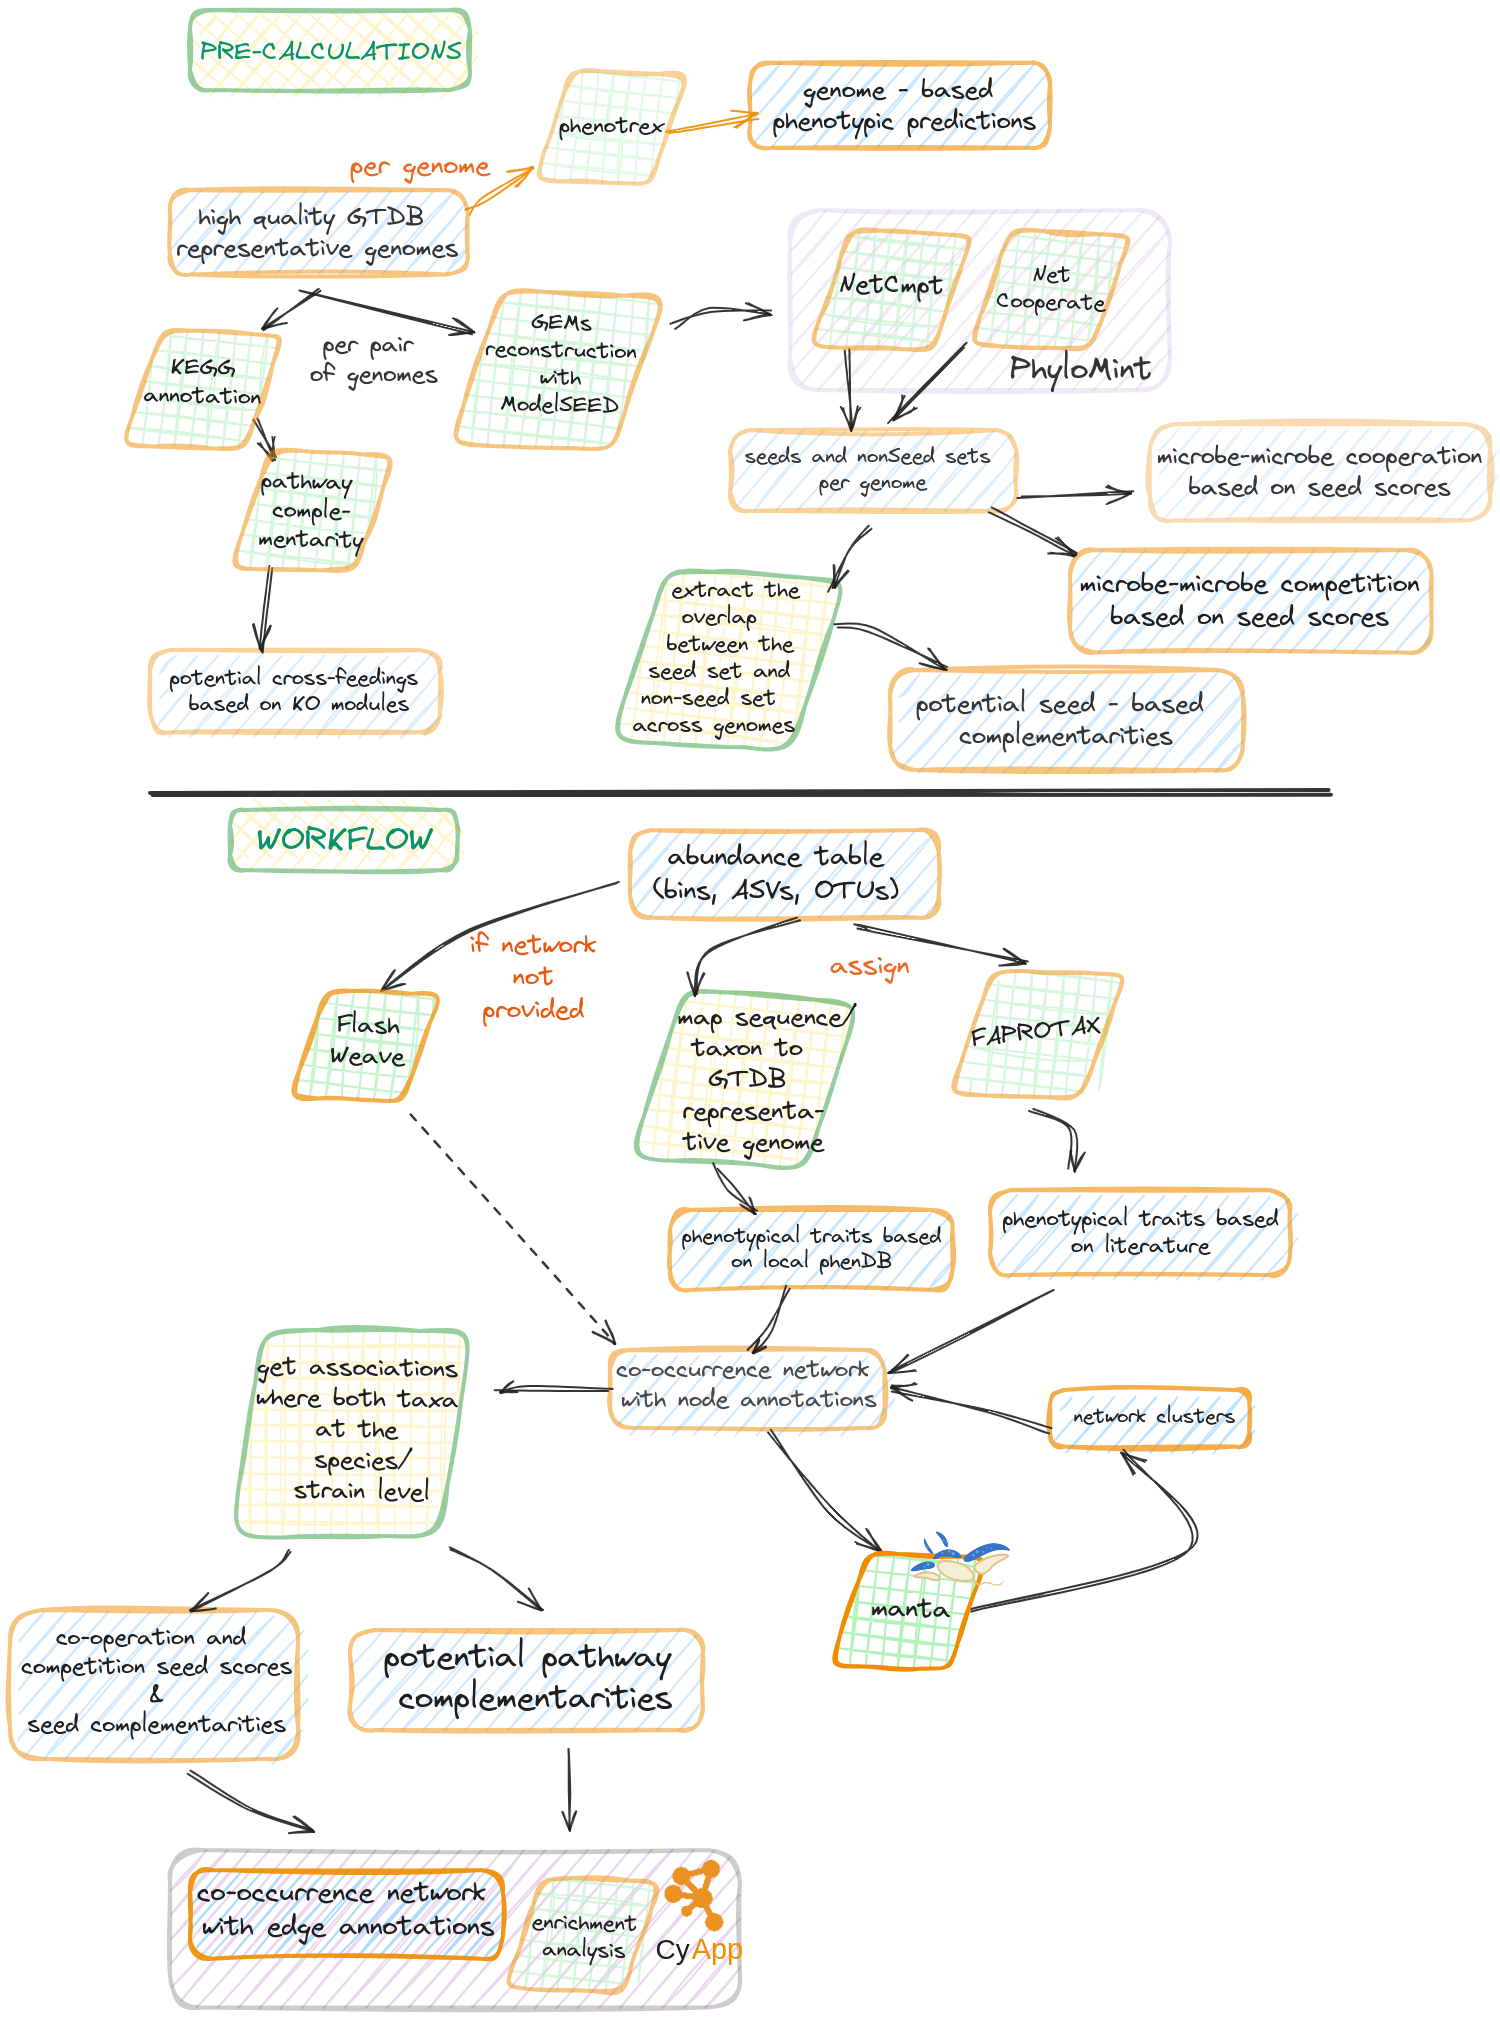
\includegraphics[width=0.9\columnwidth]{figs/microbetag-wf.png}
            \caption{
                Diagram of the microbetag pre - calculations and the on the fly workflow. 
                GTDB v207 representative genomes were filtered and for those of high-quality
                33 phenotypic traits were predicted using~\texttt{phenotrex}~\cite{feldbauer2015prediction}.
                To this end, models were re-trained to sync with recent version of eggNOG~\cite{huerta2019eggnog}.
            }
        \end{figure}


        microbetag in numbers:
        $34,608$ GTDB representative genomes
        $32$ phen-model-oriented metabolic functions 
        $92$ FAPROTAX functions
        $341,568$ unique complements involved in $>184$ million beneficiary - donor pairs' complementarities
        $30,755$ GENREs leading to $~1$ billion competition and complementarity scores
        
        annotated network returned in \texttt{.cyjs} format


        For a computationally efficient way to annotate large networks, a Docker image is provided so the user runs a taxonomy assignment using the IDTAXA algorithm~\cite{murali2018idtaxa} of the DECIPHER R package~\cite{wright2016using}.
        A co-occurrence network is also built using FlashWeave~\cite{flashweave_cite}, as microbetag also does. 
            

        

    \subsection*{microbetag CytoscapeApp}
    \label{subsec:cytoapp}

        Overall comment, the CytoscapeApp returns averages and s.d. for example in seed scores. 
        If you want the exact values, go through the API. 

        % -----------
        % stats table
        % -----------
        \begin{table}[ht]

            \centering

            \begin{adjustbox}{width=1.3\textwidth,center=\textwidth}

            \begin{tabular}{c|c}

                \begin{tabular}{ccc}

                    \multicolumn{3}{c}{A. GTDB-tk: 480 bins} \\
                    \toprule
                    Step &  Time(sec) & Notes \\
                    \toprule

                    Taxonomy mapping & Cell 1,2 & on the fly \\

                    Network inference & Cell 2,2 & on the fly  \\

                    microbetag annotations & Cell 3,2 & on the fly \\

                    manta clustering & Cell 4,2 & on the fly \\

                \end{tabular} &

                \begin{tabular}{ccc}

                    \multicolumn{3}{c}{B. GTDB 16S: 3000 ASVs} \\
                    \toprule
                    Step &  Time(sec) & Notes \\
                    \toprule

                    Taxonomy assignment &  & Docker image on HP\protect\footnotemark \\

                    Taxonomy mapping & Cell 1,2 & Cell 1,3 \\

                    Network inference & Cell 2,2 & Cell 2,3 \\

                    microbetag annotations & Cell 3,2 & Cell 3,3 \\

                    manta clustering & Cell 4,2 & Cell 4,3 \\

                \end{tabular} \\
                \\
                \hline
                \\
                \begin{tabular}{ccc}

                    \multicolumn{3}{c}{C. Silva: } \\
                    \toprule
                    Step &  Time(sec) & Notes \\
                    \toprule

                    Taxonomy mapping & Cell 1,2 & Cell 1,3 \\

                    Network inference & Cell 2,2 & Cell 2,3 \\

                    microbetag annotations & Cell 3,2 & Cell 3,3 \\

                    manta clustering & Cell 4,2 & Cell 4,3 \\

                \end{tabular} &

                \begin{tabular}{ccc}

                    \multicolumn{3}{c}{D. fuzzywuzzy: } \\
                    \toprule
                    Step &  Time(sec) & Notes \\
                    \toprule

                    Taxonomy mapping & Cell 1,2 & Cell 1,3 \\

                    Network inference & Cell 2,2 & Cell 2,3 \\

                    microbetag annotations & Cell 3,2 & Cell 3,3 \\

                    manta clustering & Cell 4,2 & Cell 4,3 \\

                \end{tabular} \\

            \end{tabular}

            \end{adjustbox}

            \caption{
                Computating times per step using an abundance table of 400 taxa with taxonomy: 
                A. taxonomy scheme 
                B. 
                C.
                D. 
                \protect\footnotemark[\value{footnote}] specs of the laptop used.
            }
            
            \label{tab:grid}
        \end{table}

        The app was based on the StringApp and supported by the NRNB group.


    \subsection*{Validation of microbetag potential}
    \label{subsec:validation}


        vitamin dataset~\cite{hessler2023vitamin}

        Metagenomic or metabarcoding data are often used to predict microbial interactions in complex communities, but these predictions are rarely explored experimentally. 
        Here, we use an organism abundance correlation network to investigate factors that control community organization in mine tailings-derived laboratory microbial consortia grown under dozens of conditions.

        The network is overlaid with metagenomic information about functional capacities to generate testable hypotheses.


    \subsection*{Interpetating a real-world network with microbetag}
    \label{subsec:usecase}


        Annelies' dataset. 







\section{Discussion}
\label{sec:discussion}

    \footnote{
        The user interface should be described and a discussion of the intended uses of the software, and the benefits that are envisioned, should be included, 
        together with data on how its performance and functionality compare with, and improve, on functionally similar existing software. 
        A case study of the use of the software may be presented. The planned future development of new features, if any, should be mentioned.
    }
    




\section{Conclusions}
\label{sec:conclusions}

    \footnote{
        This should state clearly the main conclusions and provide an explanation of the importance and relevance of the case, data, opinion, database or software reported.
    }

    Data integration 




\backmatter



\bmhead{Supplementary information}
    \label{supplementary-files}
    \footnote{
        If your article has accompanying supplementary file(s) please state so here.
        E.g. supplementary figures and tables captions. 
    }



% ====================================================
% Declarations
% ====================================================
\section*{Declarations}


    \begin{itemize}

        \item \textbf{Availability of data and materials}

            \begin{itemize}
                \item Raw sequences for the use case: 
                \item Raw data for the validations case:
            \end{itemize}

        \item \textbf{Funding}
        
            This work was initiated thanks to an EMBO Scientific Exchange Grant to HZ. 
            It was then supported by the 3D’omics Horizon project (101000309). 
            We would also like to thank the National Resource for Network Biology (NRNB) and the Google Summer of Code 2023 for the support of E.I.M.D.

        \item \textbf{Conflict of interest/Competing interests} 

            The authors declare that they have no other competing interests.

        \item \textbf{Authors' contributions}
            \footnote{Based on the \href{https://www-elsevier-com.kuleuven.e-bronnen.be/researcher/author/policies-and-guidelines/credit-author-statement}{CRediT system}. Current list is indicative.}

            Conceptualization: K.F.
            Methodology: K.F. and H.Z.
            Software: H.Z., E.I.M.D. and J.M
            Validation: H.Z. and K.F.
            Formal analysis: H.Z. and K.F.
            Investigation: H.Z.
            Resources: K.F., A.E. and A.G.
            Data Curation: H.Z.
            Writing - Original Draft: H.Z. and K.F. 
            Writing - Review \& Editing: all
            Visualization: H.Z.
            Supervision: K.F., H.Z. and S.M.
            Project administration: K.F.
            Funding acquisition: K.F., A.E.


        \item \textbf{Acknowledgements}

            We would like to thank Dr Christina Pavloudi and ++ for the insight on how to organise the trait groups.


        \item \textbf{Ethics approval}

            Not applicable

        \item \textbf{Consent to participate}
        
            Not applicable.

        \item \textbf{Code availability: }

            \begin{itemize}
                \item microbetagDB related scripts: \href{https://github.com/hariszaf/microbetag}{https://github.com/hariszaf/microbetag}
                \item microbetagApp and webserver: \href{https://github.com/msysbio/microbetagApp}{https://github.com/msysbio/microbetagApp}.
                \item CytoscapeApp: \href{https://github.com/ermismd/MGG/}{https://github.com/ermismd/MGG/}
                \item Validation and use case: <think of having that under the 3D'omics organization> 
                \item Documentation web-site: \href{https://hariszaf.github.io/microbetag/}{https://hariszaf.github.io/microbetag/}
            \end{itemize}

    \end{itemize}


% ====================================================
% Appendices
% ====================================================
\begin{appendices}

    \section{Background on seed scores and complementarities}
    \label{secA1}

        \subsection{Background on seed scores}

            In that case, once a seed is assured, it activates all the rest of that group.
            Therefore, a confidence level ($C$) ranging from 0 to 1, has been previously described to quantify the relevance of each seed:

            \begin{equation}
                \label{eq:confidence}
                C_i = 1 / seed's\ group\ with \ i \ size
            \end{equation}

            $C=0$ corresponds to a non-seed node, while $C=1$ represents an independent node. 



            \begin{equation}
                \label{eq:mi_complementarity}
                MI_{Complementarity} = \frac{ | SeedSet_A \cap \neg SeedSet_B | }{ | SeedSet_A \cap (SeedSet_B \cup \neg SeedSet_B) | }
            \end{equation}


            As also described in~\cite{phylomint_ms}, it is calculated as the proportion of compounds in a species' seed set that coincide with those in an other's, while also factoring in the confidence scores associated with seed compounds.

            \begin{equation}
                \label{eq:mi_competition}
                MI_{Competition} = \frac{ \sum C (SeedSet_A \cap SeedSet_B) }{ \sum{ C (SeedSet_A )} }
            \end{equation}


        \subsection{Background on pathway complementarity}

            For example, the definition of the D-Galacturonate degradation in Bacteria (\href{https://www.genome.jp/dbget-bin/www_bget?M00631}{M00631}) is: \vspace{0.35cm}


            \makebox[1in][l]{K01812 K00041 (K01685,K16849+K16850) K00874 (K01625,K17463)}
            
            % \vspace{0.25cm}
            \begin{flushleft}
                that once breaking down, it leads to 4 alternative sets of KOs (pathways):\vspace{0.25cm}
            \end{flushleft} 

            K01812 K00041 K01685 K00874 K01625\vspace{0.25cm}

            K01812 K00041 K16849+K16850 K00874 K01625\vspace{0.25cm}

            K01812 K00041 K01685 K00874 K17463\vspace{0.25cm}

            K01812 K00041 K16849+K16850 K00874 K17463\vspace{0.5cm}


        \subsection{Complementarities}
            
            KEGG compound 
            ModelSEED compounds
            ModelSEED compounds mapped to KEGG compounds and kept only those related to KEGG modules. 


\end{appendices}


% ======================
% Bibliography
% ======================
\bibliography{sn-bibliography}


\end{document}








% ----------------------- TABLES ----------------------
% \section{Tables}\label{sec5}

% Tables can be inserted via the normal table and tabular environment. To put
% footnotes inside tables you should use \verb+\footnotetext[]{...}+ tag.
% The footnote appears just below the table itself (refer Tables~\ref{tab1} and \ref{tab2}). 
% For the corresponding footnotemark use \verb+\footnotemark[...]+

% \begin{table}[h]
% \caption{Caption text}\label{tab1}%
% \begin{tabular}{@{}llll@{}}
% \toprule
% Column 1 & Column 2  & Column 3 & Column 4\\
% \midrule
% row 1    & data 1   & data 2  & data 3  \\
% row 2    & data 4   & data 5\footnotemark[1]  & data 6  \\
% row 3    & data 7   & data 8  & data 9\footnotemark[2]  \\
% \botrule
% \end{tabular}
% \footnotetext{Source: This is an example of table footnote. This is an example of table footnote.}
% \footnotetext[1]{Example for a first table footnote. This is an example of table footnote.}
% \footnotetext[2]{Example for a second table footnote. This is an example of table footnote.}
% \end{table}

% \noindent
% The input format for the above table is as follows:

% %%=============================================%%
% %% For presentation purpose, we have included  %%
% %% \bigskip command. please ignore this.       %%
% %%=============================================%%
% \bigskip
% \begin{verbatim}
% \begin{table}[<placement-specifier>]
% \caption{<table-caption>}\label{<table-label>}%
% \begin{tabular}{@{}llll@{}}
% \toprule
% Column 1 & Column 2 & Column 3 & Column 4\\
% \midrule
% row 1 & data 1 & data 2	 & data 3 \\
% row 2 & data 4 & data 5\footnotemark[1] & data 6 \\
% row 3 & data 7 & data 8	 & data 9\footnotemark[2]\\
% \botrule
% \end{tabular}
% \footnotetext{Source: This is an example of table footnote. 
% This is an example of table footnote.}
% \footnotetext[1]{Example for a first table footnote.
% This is an example of table footnote.}
% \footnotetext[2]{Example for a second table footnote. 
% This is an example of table footnote.}
% \end{table}
% \end{verbatim}
% \bigskip
% %%=============================================%%
% %% For presentation purpose, we have included  %%
% %% \bigskip command. please ignore this.       %%
% %%=============================================%%

% \begin{table}[h]
% \caption{Example of a lengthy table which is set to full textwidth}\label{tab2}
% \begin{tabular*}{\textwidth}{@{\extracolsep\fill}lcccccc}
% \toprule%
% & \multicolumn{3}{@{}c@{}}{Element 1\footnotemark[1]} & \multicolumn{3}{@{}c@{}}{Element 2\footnotemark[2]} \\\cmidrule{2-4}\cmidrule{5-7}%
% Project & Energy & $\sigma_{calc}$ & $\sigma_{expt}$ & Energy & $\sigma_{calc}$ & $\sigma_{expt}$ \\
% \midrule
% Element 3  & 990 A & 1168 & $1547\pm12$ & 780 A & 1166 & $1239\pm100$\\
% Element 4  & 500 A & 961  & $922\pm10$  & 900 A & 1268 & $1092\pm40$\\
% \botrule
% \end{tabular*}
% \footnotetext{Note: This is an example of table footnote. This is an example of table footnote this is an example of table footnote this is an example of~table footnote this is an example of table footnote.}
% \footnotetext[1]{Example for a first table footnote.}
% \footnotetext[2]{Example for a second table footnote.}
% \end{table}

% \vfill\eject

% In case of double column layout, tables which do not fit in single column width should be set to full text width. For this, you need to use \verb+\begin{table*}+ \verb+...+ \verb+\end{table*}+ instead of \verb+\begin{table}+ \verb+...+ \verb+\end{table}+ environment. Lengthy tables which do not fit in textwidth should be set as rotated table. For this, you need to use \verb+\begin{sidewaystable}+ \verb+...+ \verb+\end{sidewaystable}+ instead of \verb+\begin{table*}+ \verb+...+ \verb+\end{table*}+ environment. This environment puts tables rotated to single column width. For tables rotated to double column width, use \verb+\begin{sidewaystable*}+ \verb+...+ \verb+\end{sidewaystable*}+.

% \begin{sidewaystable}
% \caption{Tables which are too long to fit, should be written using the ``sidewaystable'' environment as shown here}\label{tab3}
% \begin{tabular*}{\textheight}{@{\extracolsep\fill}lcccccc}
% \toprule%
% & \multicolumn{3}{@{}c@{}}{Element 1\footnotemark[1]}& \multicolumn{3}{@{}c@{}}{Element\footnotemark[2]} \\\cmidrule{2-4}\cmidrule{5-7}%
% Projectile & Energy	& $\sigma_{calc}$ & $\sigma_{expt}$ & Energy & $\sigma_{calc}$ & $\sigma_{expt}$ \\
% \midrule
% Element 3 & 990 A & 1168 & $1547\pm12$ & 780 A & 1166 & $1239\pm100$ \\
% Element 4 & 500 A & 961  & $922\pm10$  & 900 A & 1268 & $1092\pm40$ \\
% Element 5 & 990 A & 1168 & $1547\pm12$ & 780 A & 1166 & $1239\pm100$ \\
% Element 6 & 500 A & 961  & $922\pm10$  & 900 A & 1268 & $1092\pm40$ \\
% \botrule
% \end{tabular*}
% \footnotetext{Note: This is an example of table footnote this is an example of table footnote this is an example of table footnote this is an example of~table footnote this is an example of table footnote.}
% \footnotetext[1]{This is an example of table footnote.}
% \end{sidewaystable}




% ------------------   FIGURES ---------------------

% \section{Figures}\label{sec6}

% As per the \LaTeX\ standards you need to use eps images for \LaTeX\ compilation and \verb+pdf/jpg/png+ images for \verb+PDFLaTeX+ compilation. This is one of the major difference between \LaTeX\ and \verb+PDFLaTeX+. Each image should be from a single input .eps/vector image file. Avoid using subfigures. The command for inserting images for \LaTeX\ and \verb+PDFLaTeX+ can be generalized. The package used to insert images in \verb+LaTeX/PDFLaTeX+ is the graphicx package. Figures can be inserted via the normal figure environment as shown in the below example:

% %%=============================================%%
% %% For presentation purpose, we have included  %%
% %% \bigskip command. please ignore this.       %%
% %%=============================================%%
% \bigskip
% \begin{verbatim}
% \begin{figure}[<placement-specifier>]
% \centering
% \includegraphics{<eps-file>}
% \caption{<figure-caption>}\label{<figure-label>}
% \end{figure}
% \end{verbatim}
% \bigskip
% %%=============================================%%
% %% For presentation purpose, we have included  %%
% %% \bigskip command. please ignore this.       %%
% %%=============================================%%

% \begin{figure}[h]%
% \centering
% 
\includegraphics[width=0.9\textwidth]{fig.eps}
% \caption{This is a widefig. This is an example of long caption this is an example of long caption  this is an example of long caption this is an example of long caption}\label{fig1}
% \end{figure}

% In case of double column layout, the above format puts figure captions/images to single column width. To get spanned images, we need to provide \verb+\begin{figure*}+ \verb+...+ \verb+\end{figure*}+.

% For sample purpose, we have included the width of images in the optional argument of \verb+\includegraphics+ tag. Please ignore this. 




% ----------------  ALGORITHSM ------------------------

% Packages \verb+algorithm+, \verb+algorithmicx+ and \verb+algpseudocode+ are used for setting algorithms in \LaTeX\ using the format:

% %%=============================================%%
% %% For presentation purpose, we have included  %%
% %% \bigskip command. please ignore this.       %%
% %%=============================================%%
% \bigskip
% \begin{verbatim}
% \begin{algorithm}
% \caption{<alg-caption>}\label{<alg-label>}
% \begin{algorithmic}[1]
% . . .
% \end{algorithmic}
% \end{algorithm}
% \end{verbatim}
% \bigskip
% %%=============================================%%
% %% For presentation purpose, we have included  %%
% %% \bigskip command. please ignore this.       %%
% %%=============================================%%

% You may refer above listed package documentations for more details before setting \verb+algorithm+ environment. For program codes, the ``verbatim'' package is required and the command to be used is \verb+\begin{verbatim}+ \verb+...+ \verb+\end{verbatim}+. 

% Similarly, for \verb+listings+, use the \verb+listings+ package. \verb+\begin{lstlisting}+ \verb+...+ \verb+\end{lstlisting}+ is used to set environments similar to \verb+verbatim+ environment. Refer to the \verb+lstlisting+ package documentation for more details.

% A fast exponentiation procedure:

% \lstset{texcl=true,basicstyle=\small\sf,commentstyle=\small\rm,mathescape=true,escapeinside={(*}{*)}}
% \begin{lstlisting}
% begin
%   for $i:=1$ to $10$ step $1$ do
%       expt($2,i$);  
%       newline() od                (*\textrm{Comments will be set flush to the right margin}*)
% where
% proc expt($x,n$) $\equiv$
%   $z:=1$;
%   do if $n=0$ then exit fi;
%      do if odd($n$) then exit fi;                 
%         comment: (*\textrm{This is a comment statement;}*)
%         $n:=n/2$; $x:=x*x$ od;
%      { $n>0$ };
%      $n:=n-1$; $z:=z*x$ od;
%   print($z$). 
% end
% \end{lstlisting}

% \begin{algorithm}
% \caption{Calculate $y = x^n$}\label{algo1}
% \begin{algorithmic}[1]
% \Require $n \geq 0 \vee x \neq 0$
% \Ensure $y = x^n$ 
% \State $y \Leftarrow 1$
% \If{$n < 0$}\label{algln2}
%         \State $X \Leftarrow 1 / x$
%         \State $N \Leftarrow -n$
% \Else
%         \State $X \Leftarrow x$
%         \State $N \Leftarrow n$
% \EndIf
% \While{$N \neq 0$}
%         \If{$N$ is even}
%             \State $X \Leftarrow X \times X$
%             \State $N \Leftarrow N / 2$
%         \Else[$N$ is odd]
%             \State $y \Leftarrow y \times X$
%             \State $N \Leftarrow N - 1$
%         \EndIf
% \EndWhile
% \end{algorithmic}
% \end{algorithm}



% ----------------- EQUATIONS --------------------

% \section{Equations}\label{sec4}

% Equations in \LaTeX\ can either be inline or on-a-line by itself (``display equations''). For
% inline equations use the \verb+$...$+ commands. E.g.: The equation
% $H\psi = E \psi$ is written via the command \verb+$H \psi = E \psi$+.

% For display equations (with auto generated equation numbers)
% one can use the equation or align environments:
% \begin{equation}
% \|\tilde{X}(k)\|^2 \leq\frac{\sum\limits_{i=1}^{p}\left\|\tilde{Y}_i(k)\right\|^2+\sum\limits_{j=1}^{q}\left\|\tilde{Z}_j(k)\right\|^2 }{p+q}.\label{eq1}
% \end{equation}
% where,
% \begin{align}
% D_\mu &=  \partial_\mu - ig \frac{\lambda^a}{2} A^a_\mu \nonumber \\
% F^a_{\mu\nu} &= \partial_\mu A^a_\nu - \partial_\nu A^a_\mu + g f^{abc} A^b_\mu A^a_\nu \label{eq2}
% \end{align}
% Notice the use of \verb+\nonumber+ in the align environment at the end
% of each line, except the last, so as not to produce equation numbers on
% lines where no equation numbers are required. The \verb+\label{}+ command
% should only be used at the last line of an align environment where
% \verb+\nonumber+ is not used.
% \begin{equation}
% Y_\infty = \left( \frac{m}{\textrm{GeV}} \right)^{-3}
%     \left[ 1 + \frac{3 \ln(m/\textrm{GeV})}{15}
%     + \frac{\ln(c_2/5)}{15} \right]
% \end{equation}
% The class file also supports the use of \verb+\mathbb{}+, \verb+\mathscr{}+ and
% \verb+\mathcal{}+ commands. As such \verb+\mathbb{R}+, \verb+\mathscr{R}+
% and \verb+\mathcal{R}+ produces $\mathbb{R}$, $\mathscr{R}$ and $\mathcal{R}$
% respectively (refer Subsubsection~\ref{subsubsec2}).
